\section{Rück- und Ausblick}
Soll/Ist Vergleich
Lessons Learned (User Umfrage nutzen)
\subsection{Zukünftige Entwicklung}
\textbf{Arduino:}Als Erweiterungen für den Arduino sollen in Zukunft noch eine Alarmsirene vom Typen BSE128 verbaut werden und für die Standorterkennung noch die Google API zur beseren Lokalisierung genutzen werden. 
Für die Sirene muss das Gesamtsystem noch dahingehend erweitert werden, dass eine Kommunikation zum Arduino hin möglich wird. Auf dem Arduino muss hierfür noch realisiert werden, dass der Rückgabewert vom Server abgespeichert wird und in regelmäßigen Abständen geprüft wird, dass sich das Gerät nicht aus dem vom Anwender definierten Bereich entfernt hat. Es muss also noch Geofencing ermöglicht werden, um zu erkennen wann die Sirene auslösen soll. Es ist aber auch eine einfache Lösung denkbar, bei der der Benutzer den Alarm aus der Entfernung selbst steuern muss bzw kann.

Aus Hardware Sicht muss dann nur die Sirene mittels Transistorschaltung an den Arduino angeschlossen und mit Strom versorgt werden, damit der Arduino das Alarmsignal im Fall einer Entwendung geben kann. Die Schaltung dafür sieht wie folgt aus:
\begin{figure} [H]
	\begin{center}
		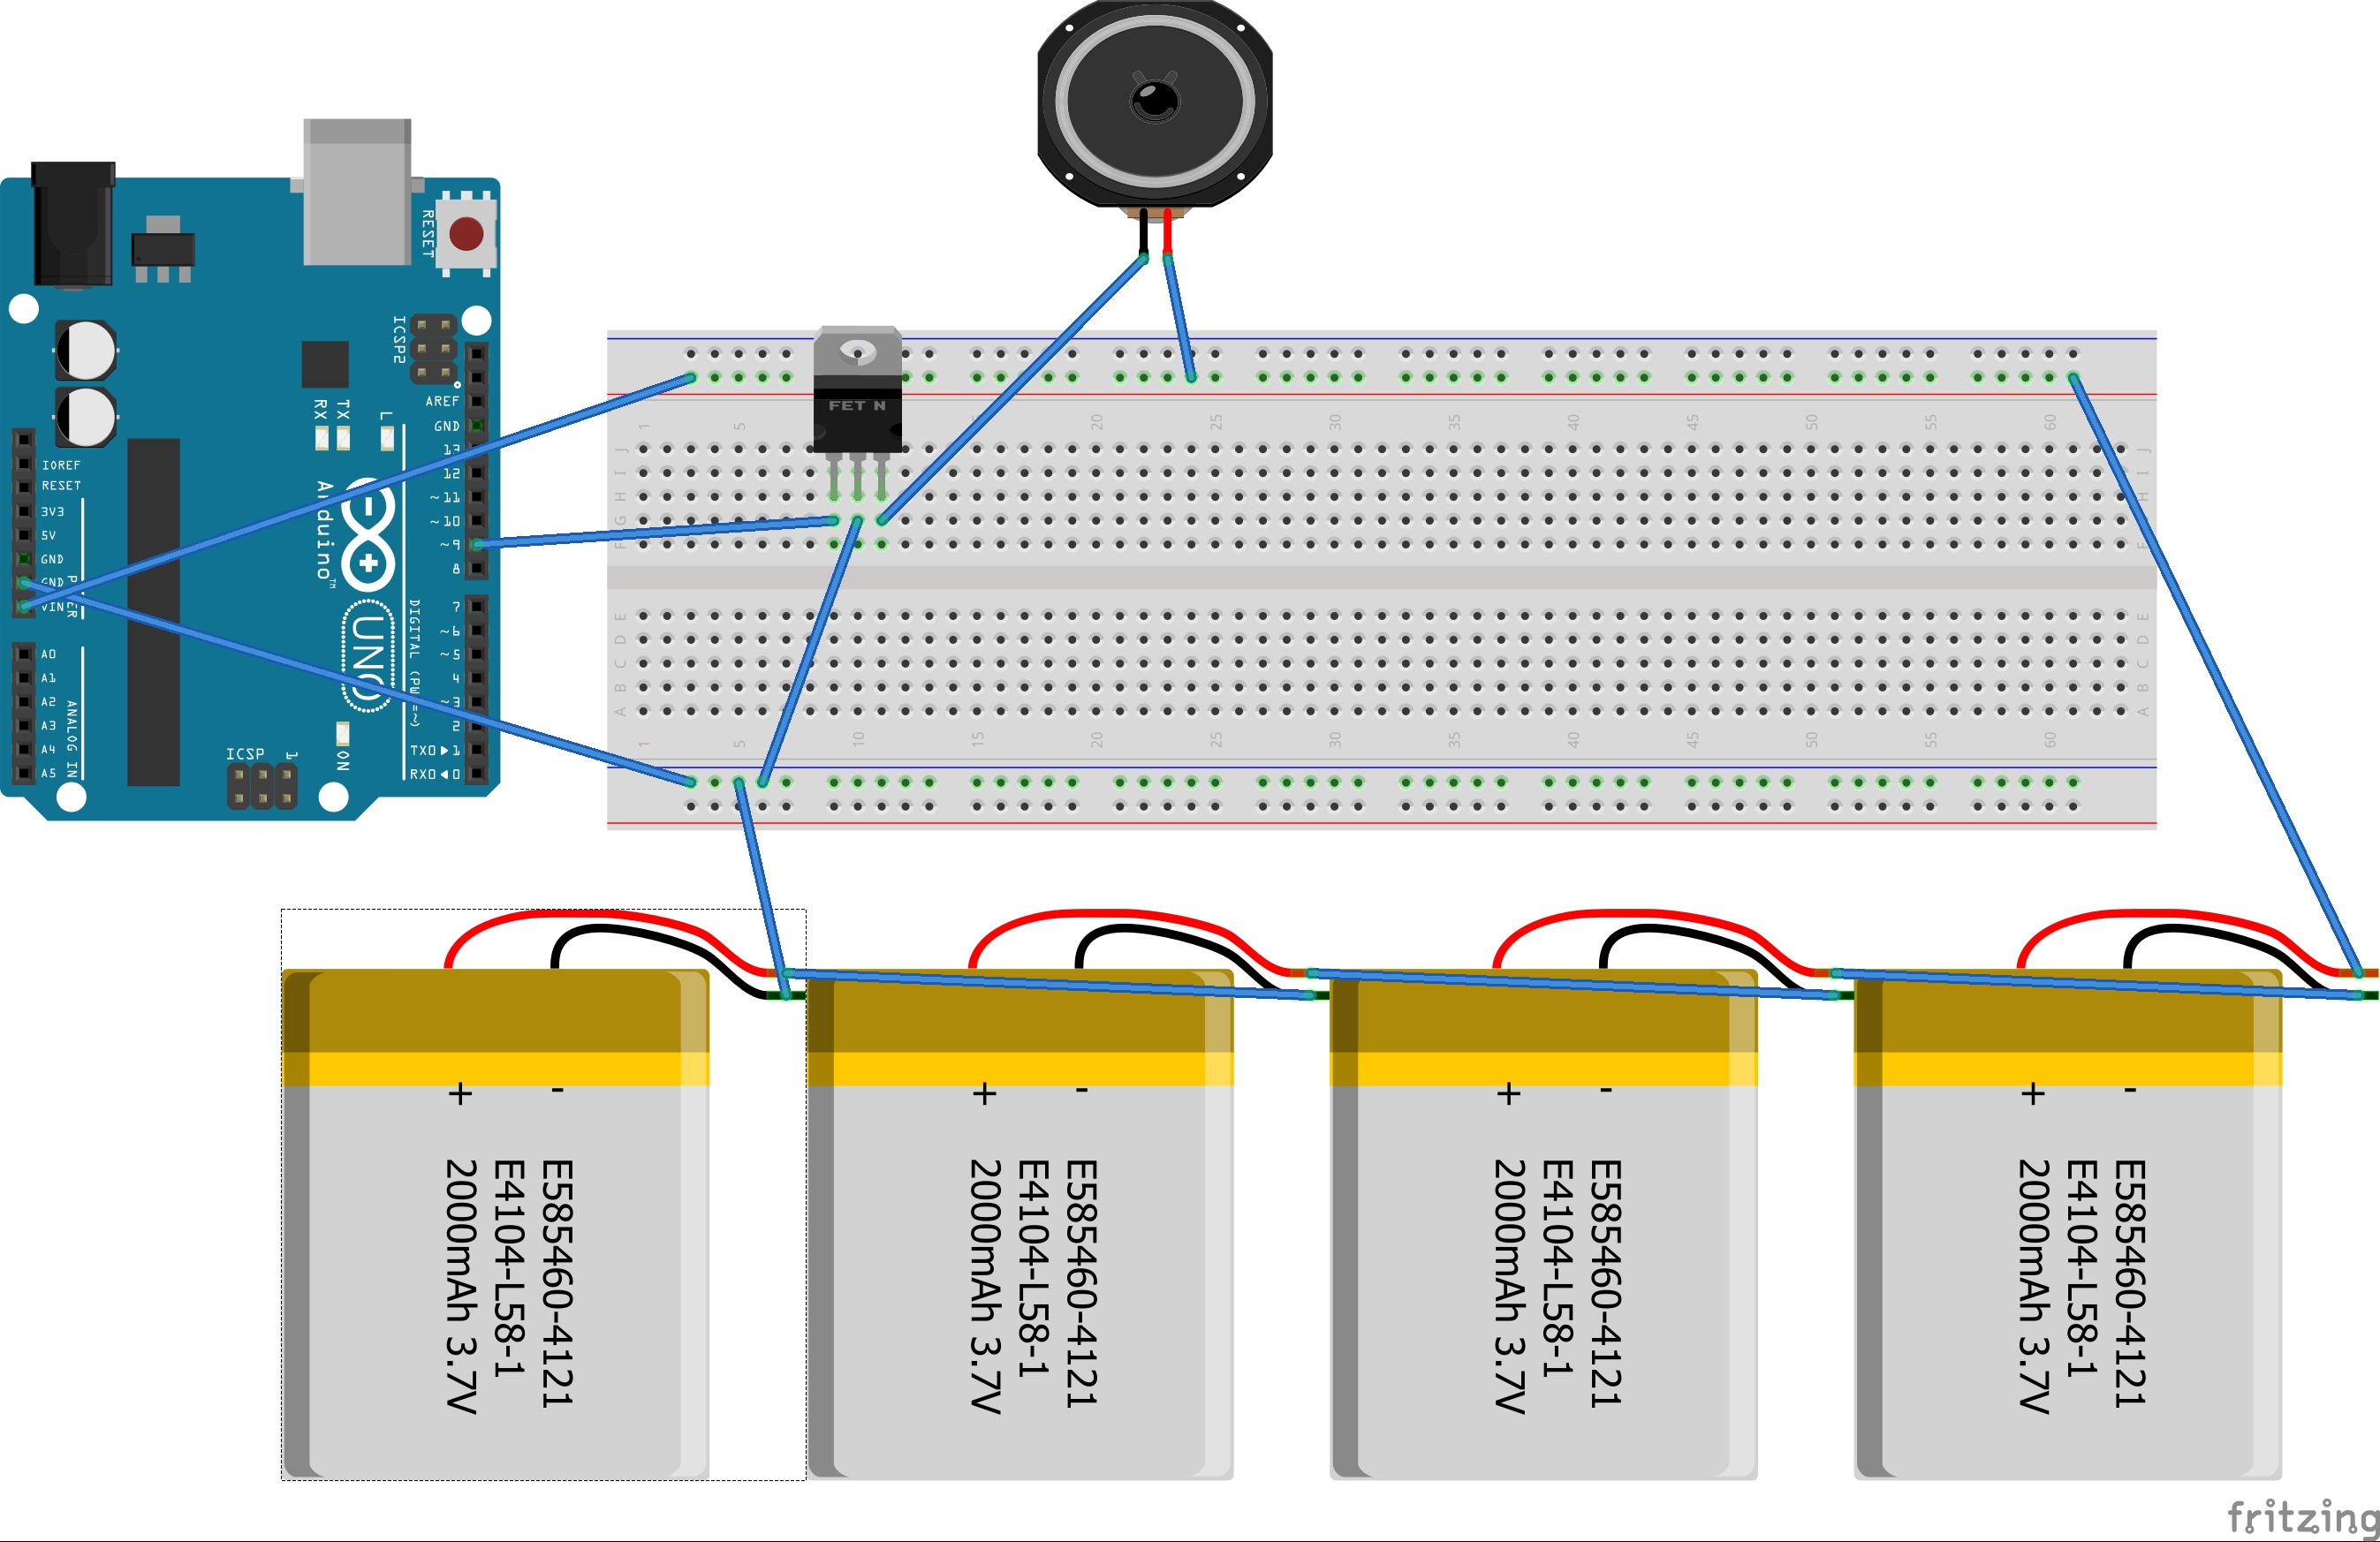
\includegraphics[width=1\textwidth]{Bilder/Arduino_Sirene.jpg}
		\caption{Systemerweiterung um Sirene}
		\label{sirene}
	\end{center}
\end{figure}
Dabei kann die Sirene, da sie 12-24V Eingangsspannung akzeptiert, an die Stromversorgung des Arduinos mit angeschlossen werden. Es muss dafür jedoch eventuell die Akkuleistung ebenfalls erweitert werden. Dies muss jedoch erst noch getestet werden. 

Die Sirene soll zukünftig durch eine einfache N-Channel Mosfet Schaltung gesteuert werden.
Um den Google Standort Service effektiv verwenden zu können, ist die Erweiterung um einen WLAN Empfänger sinnvoll. Somit kann neben den Informationen, die durch GSM und GPS zur Verfügung stehen, auch die lokalen WLAN-Netze zur Standortermittlung genutzt werden. Dies erhöht weiter die Genauigkeit kann aber theoretisch auch wegfallen. Die Verwendung der API ist jedoch kostenpflichtig und dementsprechend ist das Geschäftskonzept eventuell weiter zu überdenken. Eine mögliche Lösung hierfür wäre ein monatliches Bezahlkonzept, über das man je nach Bedarf die API Standorterkennung hinzu buchen kann.




\textbf{Webserver} 
\\
\textit{Finalisierung der Verschlüsselung}
Der erste Punkt, der in Zukunft bearbeitet werden soll, ist die vollständige Implementierung und ein anschließendes Testen der Verschlüsselung der Nutzdaten. Für den Webserver ist wie zuvor beschrieben bereits alles fertig. Es gilt nun also die entsprechend umgekehrten Abläufe in den beiden Apps zu realisieren.

Darüber hinaus sollte geprüft werden, ob es auch möglich ist, die Koordinaten bereits auf dem Arduino zu verschlüsseln. So könnte zusätzliche Sicherheit der Daten gewonnen werden.
\\
\textit{Umstellung auf HTTPS}
Bei der Entwicklung der iOS-App trat an der Stelle des Auslesens der JSON codierten Daten ein Problem auf. Die Fehlermeldungen waren zunächst nicht eindeutig zu interpretieren, doch es stellte sich heraus, dass mit der von uns gewählten Version nur von HTTPS-Seiten JSONs mittels HTTP-GET abgefragt werden können.

Um derartige Probleme in Zukunft zu umgehen, soll der Webserver von HTTP auf HTTPS umgestellt werden. Wir hatten auch erst überlegt, dies im aktuellen Bearbeitungszeitraum umzusetzen, jedoch fand sich für die iOS-App eine Alternativlösung. Auch erste Recherchen zur Umstellung auf HTTPS zeigten uns, dass dies doch ziemlich aufwendig werden und wieder neue Probleme mit sich bringen könnte.
\\
\textit{Bidirektionale Kommunikation ermöglichen}
Ein weiteres Feature, das in Zukunft realisiert werden soll, ist eine Kommunikation auch in die andere Richtung. Es soll also dann möglich sein, dass die App Befehle oder sonstige Daten an den Webserver schickt und der Arduino diese dann auch abfragen kann. Eine solche Kommunikation wäre zum Beispiel für das Aktivieren der ebenfalls noch geplanten Sirene im Innenraum des Fahrzeugs erforderlich.
\\
\textit{MQTT als redundanten Übertragungsweg einrichten}
Um nicht nur den bisherigen Übertragungsweg über den HTTP-Server nutzen zu können und somit anfällig für Systemausfälle zu sein, soll ein zweiter, redundanter Übertragungsweg mit Hilfe des MQTT-Protokolls errichtet werden. Hierfür ist als erstes das Bereitstellen eines eigenen MQTT-Brokers erforderlich, um direkt unabhängig von Dritten zu sein. Auch muss ein MQTT-Topic definiert werden, in welchem die Kommunikation stattfinden soll. Im nächsten Schritt muss auf dem Arduino ein entsprechendes Skript programmiert werden, mit welchem die Koordinaten mittels PUBLISH zum MQTT-Broker übermittelt werden können. Dieses muss dann entweder parallel zum bisherigen Skript ausgeführt werden oder es werden beide in einem neuen Skript vereinigt.

 Anschließend muss in den beiden Apps ein MQTT-SUBSCRIBE implementiert werden, um die vom Arduino veröffentlichten Daten zu erhalten. Auch dies muss parallel zur Datenabfrage vom Webserver geschehen. Zusätzlich soll in den Apps dann ein Abgleich beider Daten (HTTP und MQTT) implementiert werden. Sind beide Daten gleich werden die neuen Koordinaten übernommen. Für den anderen Fall, dass die beiden Datenpakete unterschiedlich sind, muss noch überprüft werden, welche Daten dann gespeichert werden. 
 \\
\textbf{Android} 
Im Großen und Ganzen war das Projekt eine neue Erfahrung, sowohl das Zusammenarbeiten oder auch die neuen technischen Kenntnisse, die man sich im erlernt hat.
Was man bis jetzt erreicht hat, ist ein großer Schritt. Die App ist designtechnisch sehr fortgeschritten. Die Technik dahinter funktioniert. Version 1 hat alle mindesten Anforderungen erfüllt.
Für den nächsten Versionen sollten mehr Möglichkeiten eine Datenbank Einbindung mit "Firebase", um die Datenbankverwaltung besser zu verwalten. Im Design der App konnten Verbesserungen durchgeführt werden..

\\
\textbf{iOS} Moni